\documentclass{article}

\usepackage[english]{babel}
\usepackage[utf8]{inputenc}
\usepackage{amsfonts}
\usepackage{fancyhdr}
\usepackage{graphicx}
\usepackage{hyperref}
\usepackage{listings}
\usepackage{titling}
\usepackage{xcolor}
\usepackage{float}

\renewcommand\maketitlehooka{\null\mbox{}\vfill}
\renewcommand\maketitlehookd{\vfill\null}

\newcommand{\currentversion}{1.0.0}

\lstdefinelanguage{fsharp} {
    morekeywords={let, new, match, with, rec, open, module, namespace, type, of, member, and, for, in, do, begin, end, fun, function, try, mutable, if, then, else},
    keywordstyle=\color{blue},
    sensitive=false,
    morecomment=[l][\color{green}]{//},
    morestring=[b]",
    stringstyle=\color{red}
}

\lstset{language=fsharp}


%extremely hacky solution right now
\author{%
    \vspace{3.5mm}\currentversion\\
    Adrián Habušta
    }
\title{%
    \LARGE Software Project Specification \\
    \Large for \\
    \Huge Reimplementation of Pygmalion \\\vspace{10mm}
    \normalsize Pygmalion was a proof of concept visual programming system
    put forward in the year 1975. It involved programming using so-called
    icons, and creating functions by remembering user actions, instead of
    writing them in code. This project focuses on creating a simple programming
    system with the same key ideas as Pygmalion.
    }
\date{May 14, 2023}

\begin{document}
    \begin{titlepage}
        \maketitle
    \end{titlepage}

    \tableofcontents
    \newpage

    \section{Basic Information}
        \subsection{Description of Software Project}
            This software project is inspired by an old programming system called Pygmalion.
            Pygmalion never moved past the prototype stage, and this project is a proof of concept that is meant
            to show how using a system with ideas borrowed from Pygmalion would be like. These ideas include
            representing data, methods and even objects with icons. Another key idea is creating methods by remembering
            user actions. This is what this project will focus on the most.

        \subsection{Used technologies}
            \begin{itemize}
                \item
                    F\# - used programming language
                \item
                    Fable - F\# to JS compiler

            \end{itemize}

        \subsection{References}
            \begin{itemize}

                \item
                    Pygmalion specification
                    \subitem
                        - \url{https://apps.dtic.mil/sti/pdfs/ADA016811.pdf}

            \end{itemize}


    \section{Detailed functionality}
        \subsection{Icon representation}
            Internally, custom icons will be stored in a Dictionary mapping from names to specific icons. The data
            will look something like this:
            \lstinputlisting{include/icon_representation_example.fs}

            \noindent
            The CustomIcon type represents a sort of "master" icon, which stores all data related to an icon. This
            means both the instructions of said icon, and also information necessary for drawing the icon to the screen.
            This is done by using the DrawnIcon, which only stores iformation used for drawing an icon.

        \subsection{Evaluation}
            Icons are evaluated by building simple trees of instructions. The instructions will look something like
            this:
            \lstinputlisting{include/icon_evaluation_example.fs}

            \noindent
            Icons will, by default, only contain a Trap, which when hit during runtime, opens the icon for editing.
            During editing, operations made by the user will slowly build up an instruction tree that is stored and
            later used to evaluate instances of said icon. Using custom icons within an icon is done by saving the name
            of the icon we wish to evaluate.


    \section{Screens}
        \subsection{Single Tab}
        This is the only screen the software will feature. There will, however, exist multiple instances of this screen
        called 'tabs' that can be switched between.
        \begin{figure}[H]
            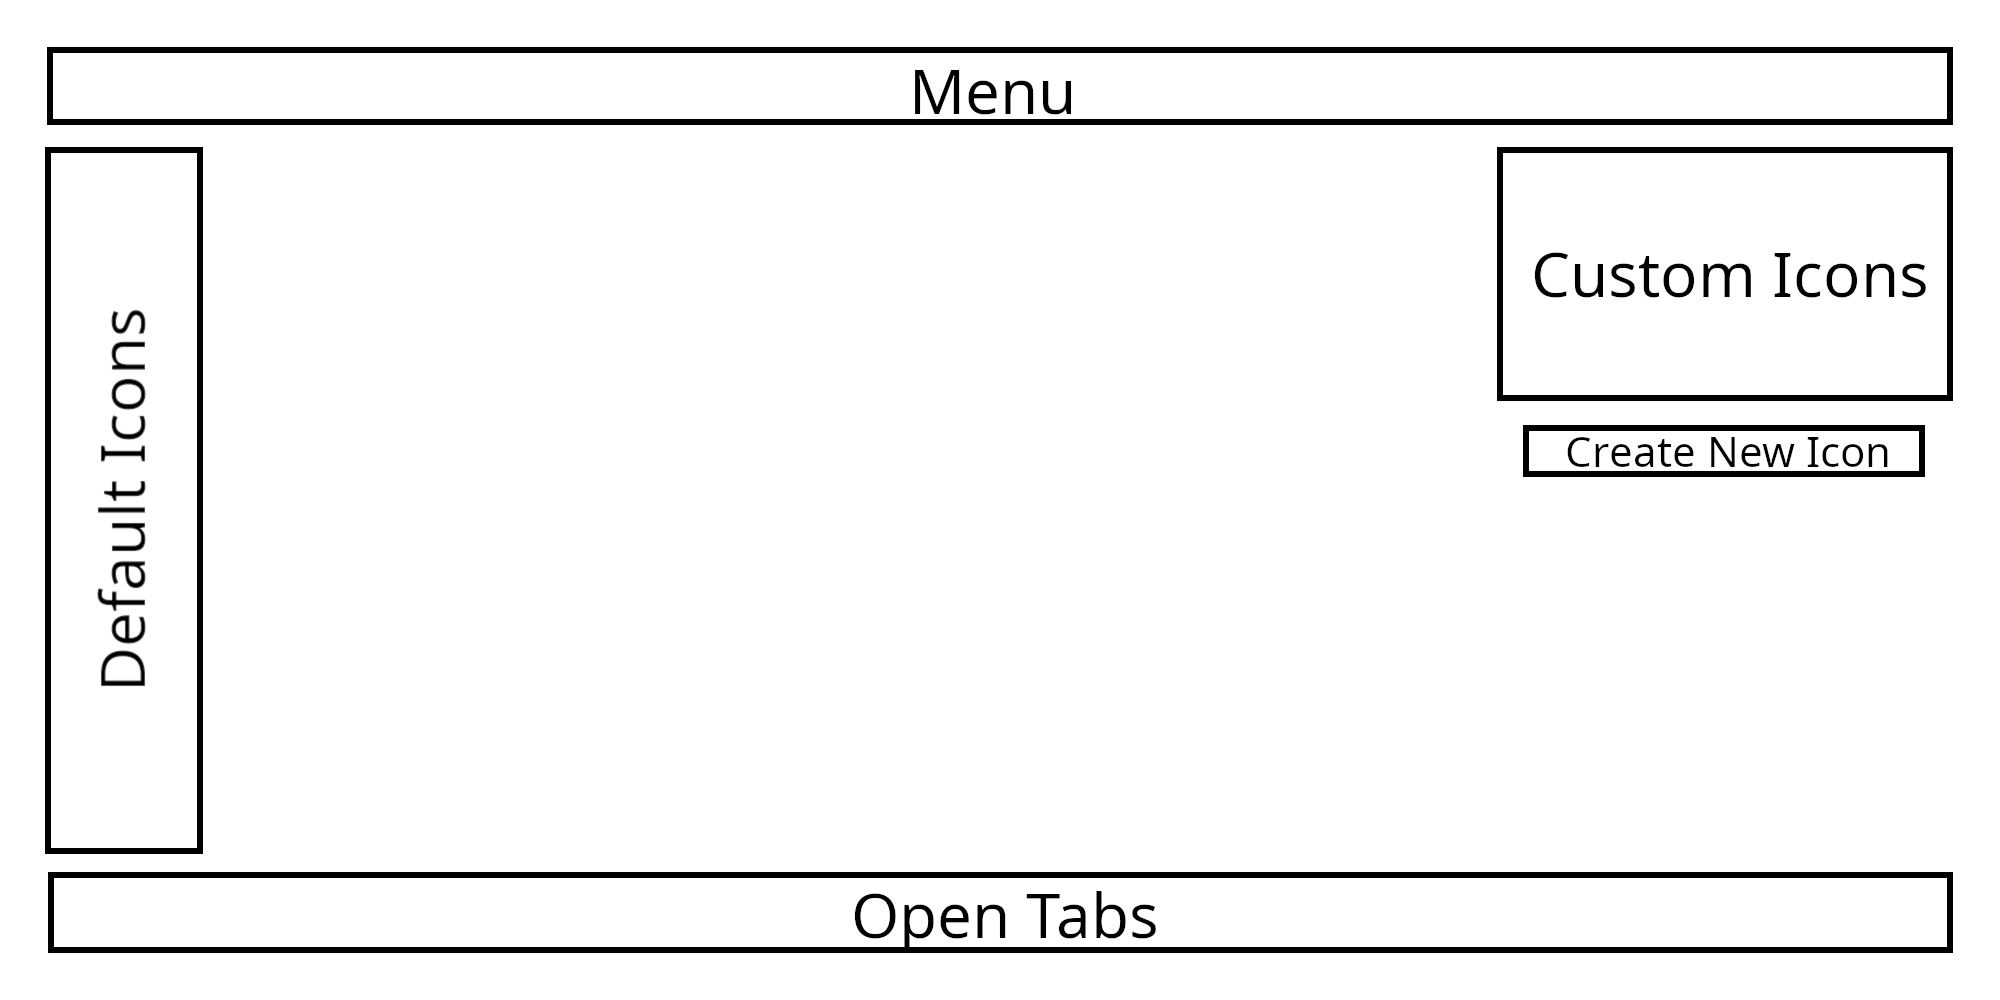
\includegraphics[width=\textwidth]{include/main_screen.png}
            \centering
        \end{figure}

        The default and custom icon menus will both be scrollable and collapsible, and the user will be able to drag
        icons from these menus to the screen to create duplicates of said icons.


    \section{Usage example - Factorial}
        This section will demonstrate how an icon which computes the factorial of a number can be created.
        \begin{itemize}
            \item
                We open the program and see the main screen
                \begin{figure}[H]
                    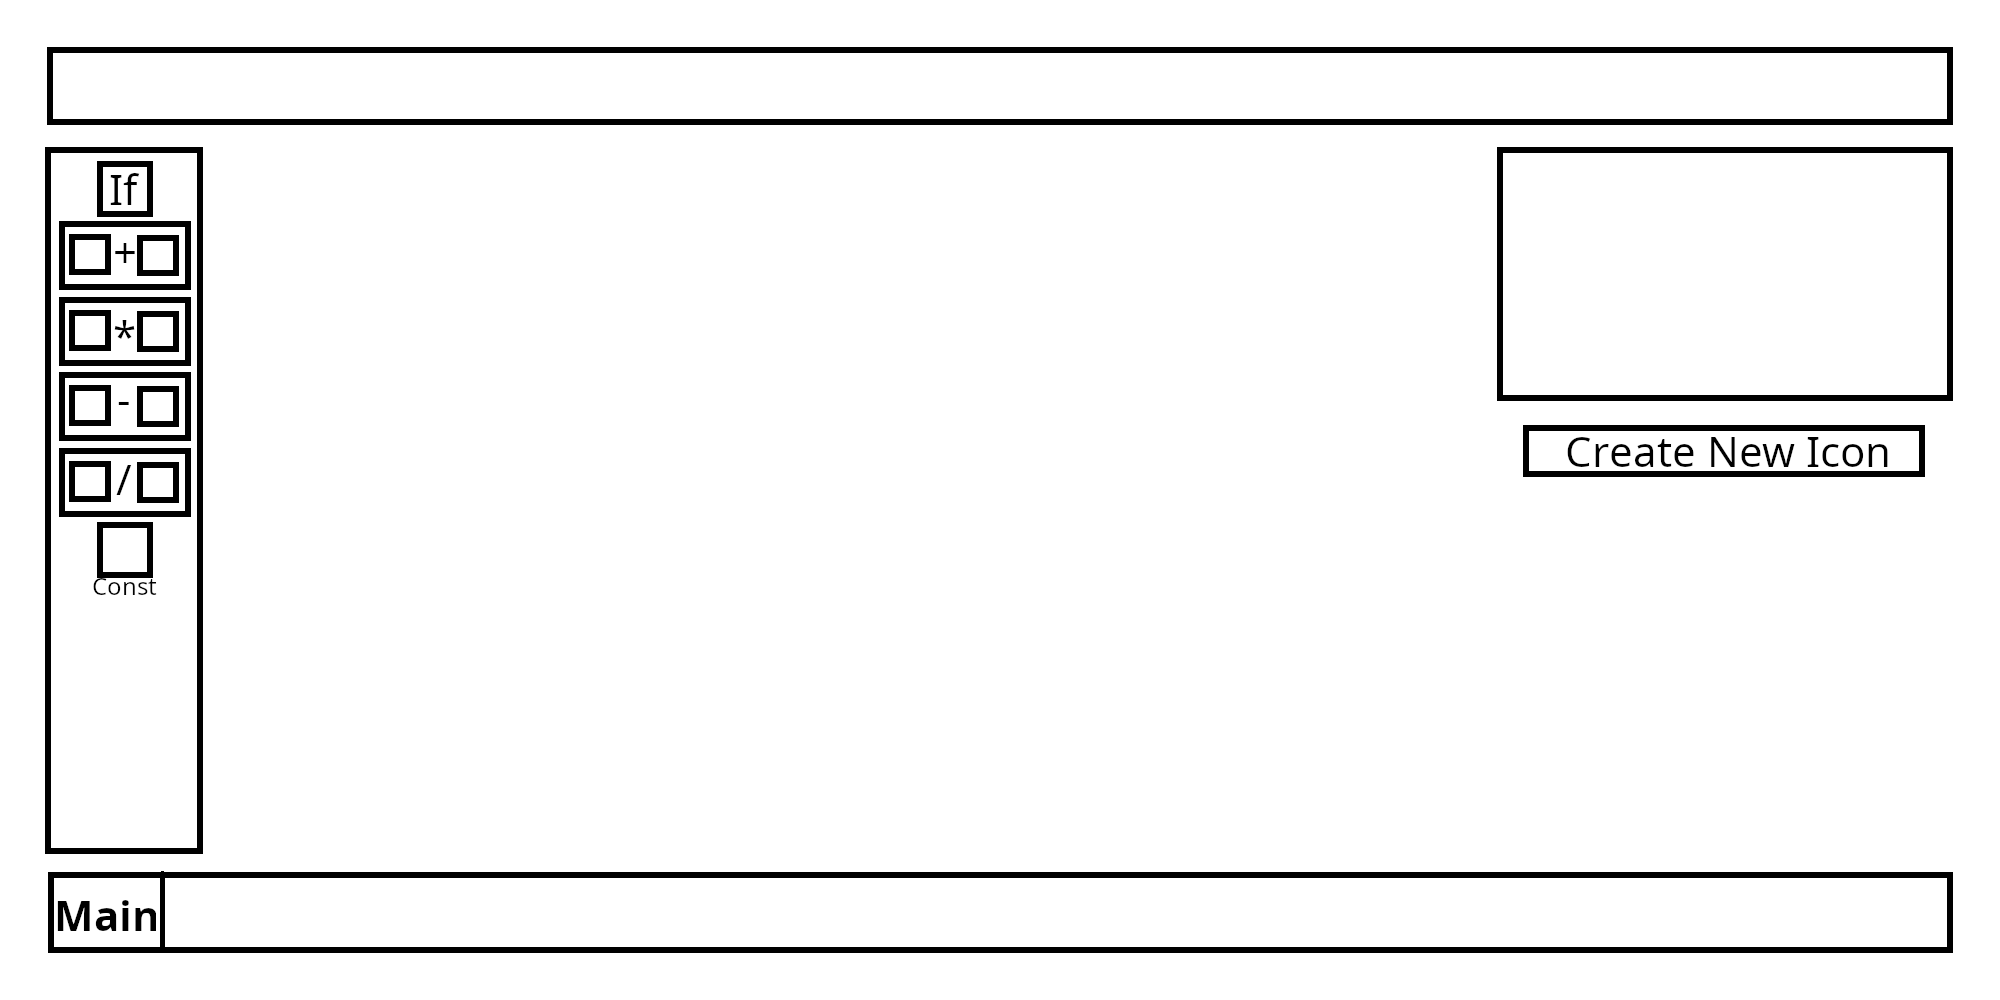
\includegraphics[width=\textwidth]{include/example_factorial_start.png}
                    \centering
                \end{figure}

            \item
                We click the \textbf{Create New Icon} button below the custom icons menu.

            \item
                We name our icon 'factorial' and set the amount of its inputs to one. This creates a new empty icon, with said name, which is added to the custom icons
                menu. This icon can than be dragged onto the field. 
                \begin{figure}[H]
                    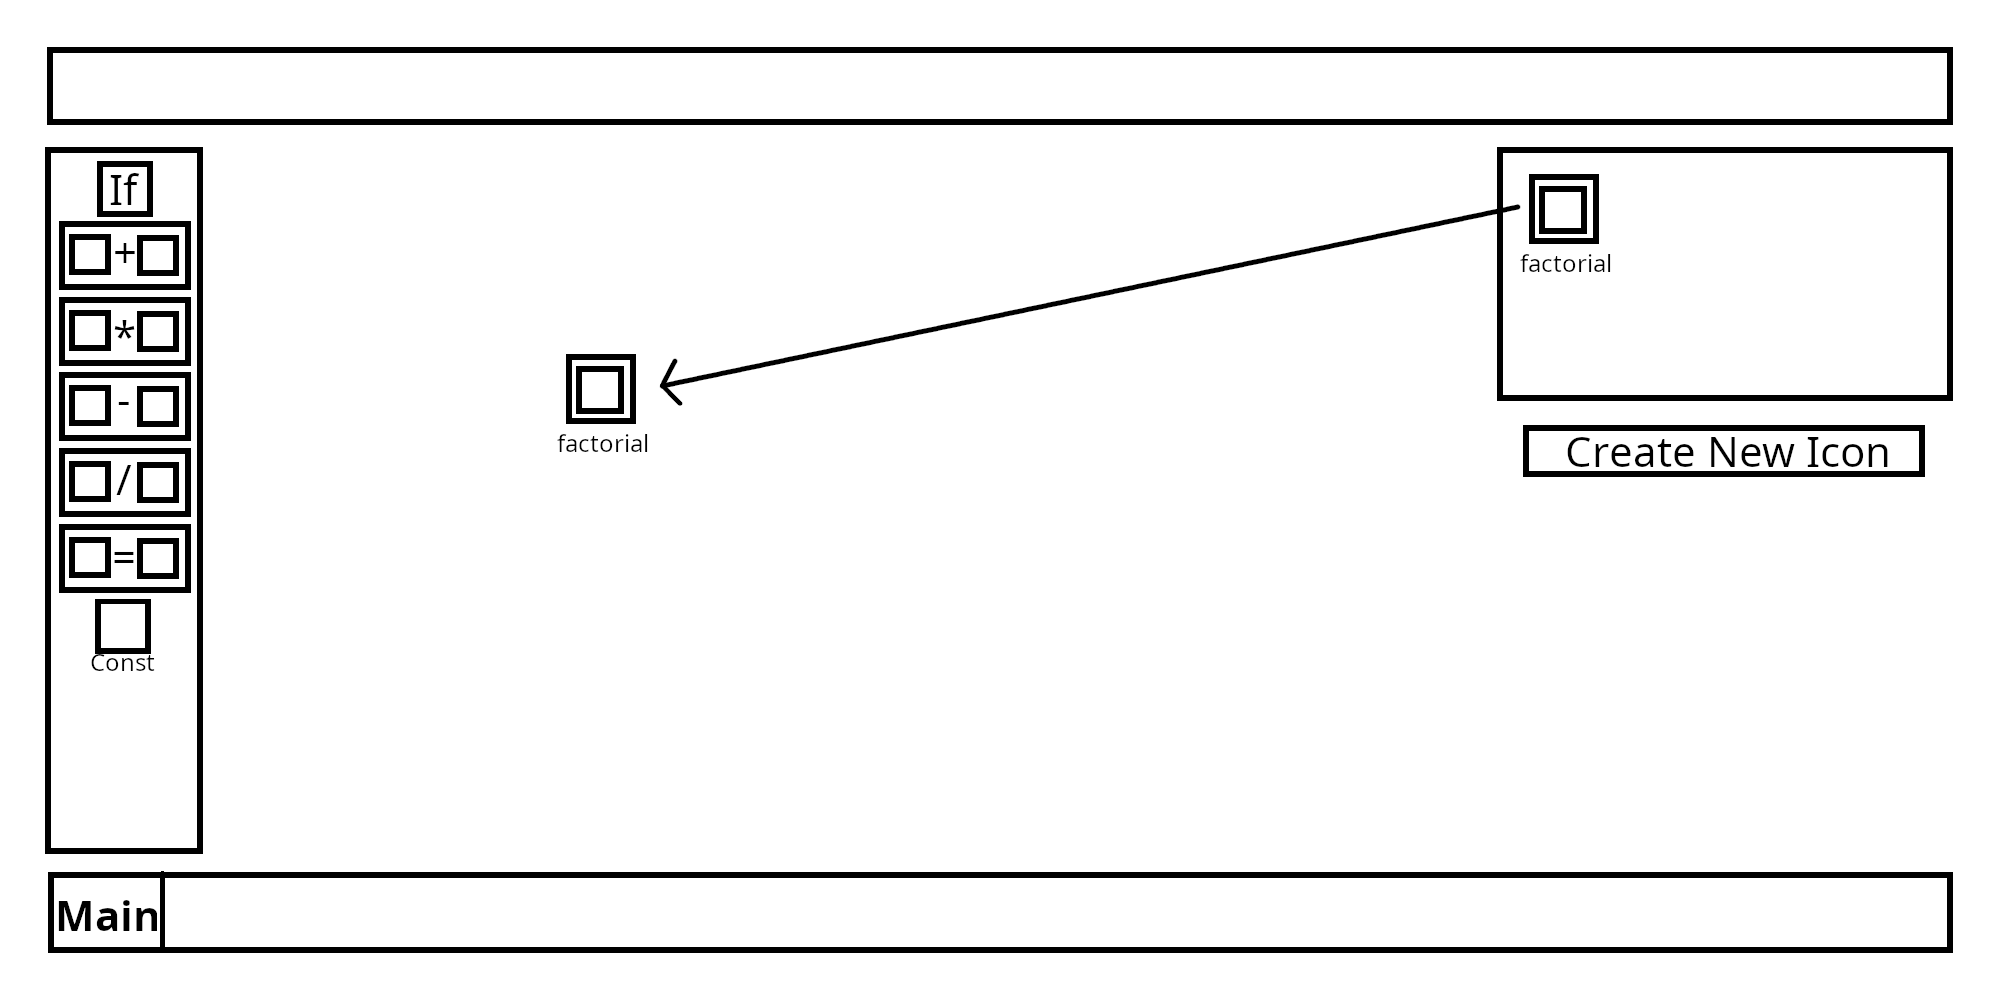
\includegraphics[width=\textwidth]{include/example_factorial_add_icon.png}
                    \centering
                \end{figure}

            \item
                With the icon on the field, we can fill its inputs with values, and then left-click on the icon to execute its
                code.

            \item
                Since the icon is new, we immediately hit a so called \textbf{trap}. This pauses execution and opens a new tab
                containing the \textbf{context} of the icon (which is mostly empty for new icons). This is where we program
                icons.
                \begin{figure}[H]
                    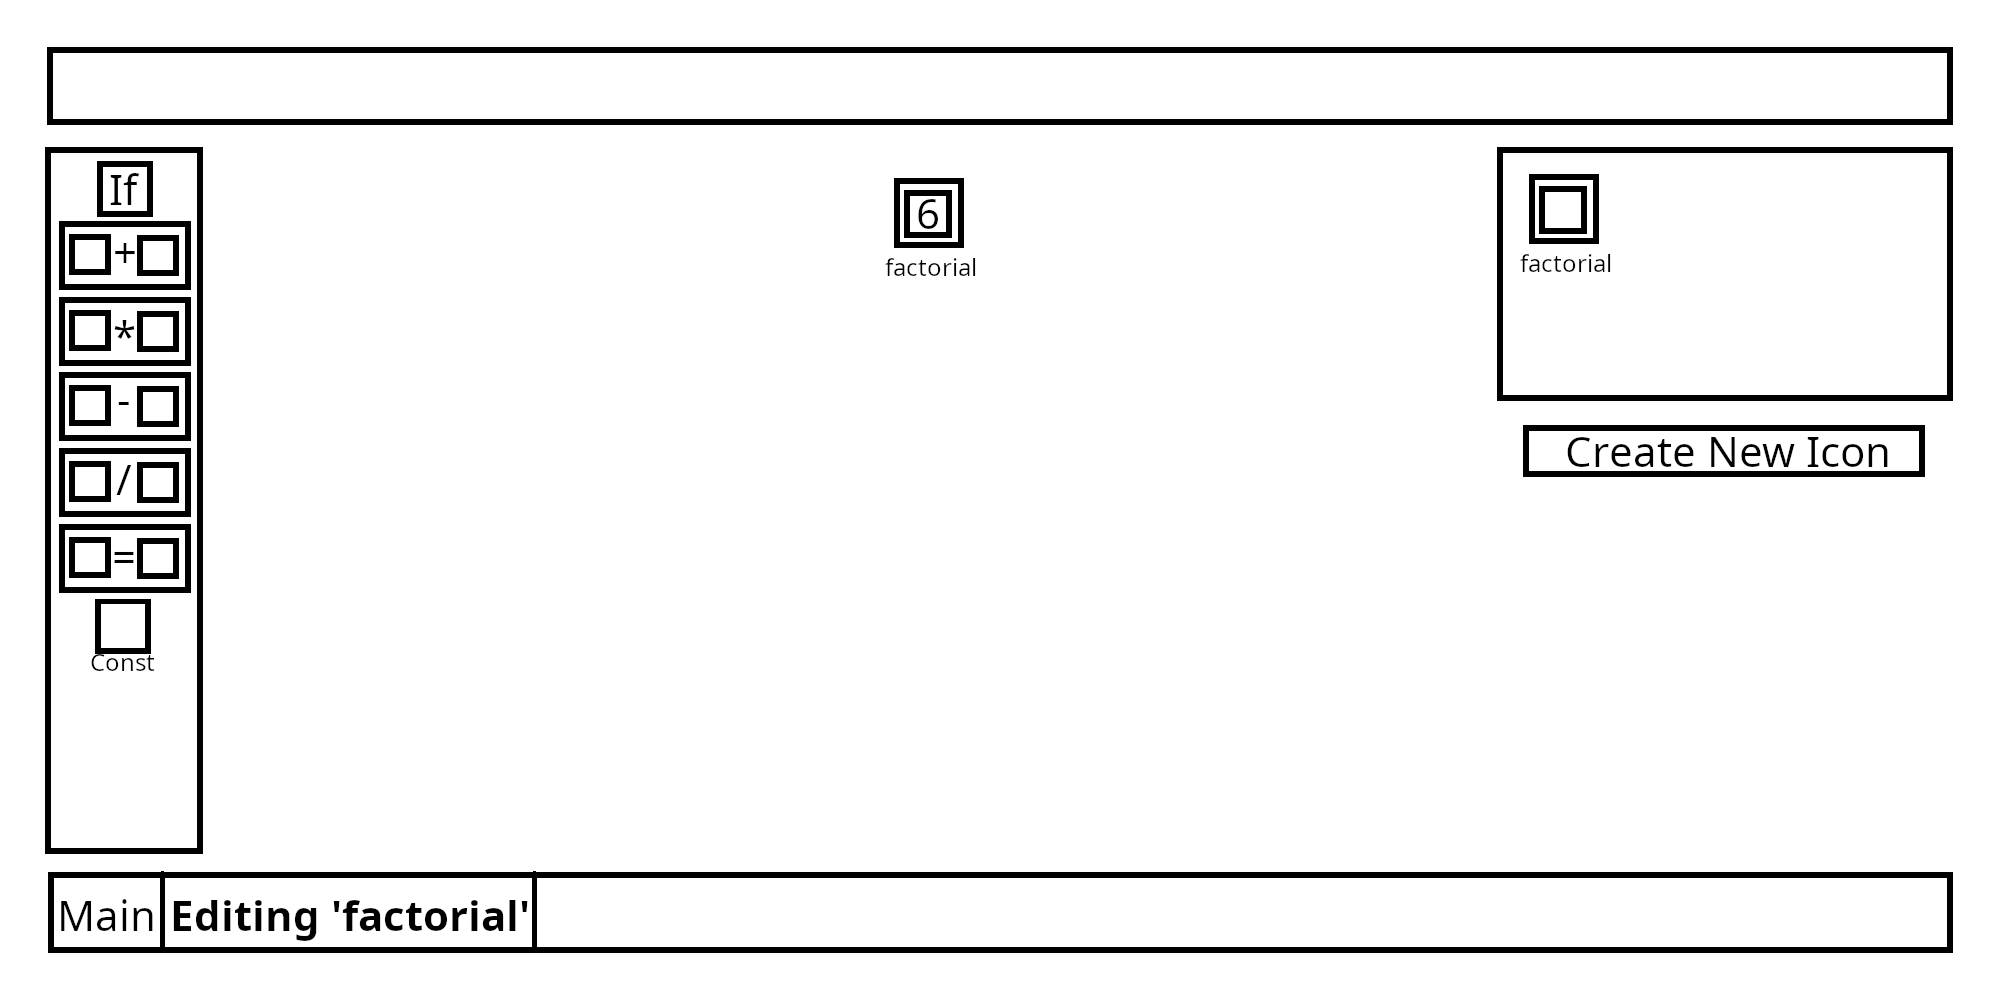
\includegraphics[width=\textwidth]{include/example_factorial_new_tab.png}
                    \centering
                \end{figure}

            \item
                The context of an icon reprents the internals of an icon. We can program an icon by dragging icons onto the
                screen, and dragging values between them. This builds up a tree of operations which will be executed anytime
                our new icon is ran.

            \item
                In the factorial, we need to use an \textbf{If} instruction to continue. We create an \textbf{IsEqual} icon and
                use it to check whether the input parameter of the factorial is equal to one. In our case, it is not, so the
                \textbf{False} branch is highlighted, which means that all following operations we do will only execute if the
                input is not equal to one.
                \begin{figure}[H]
                    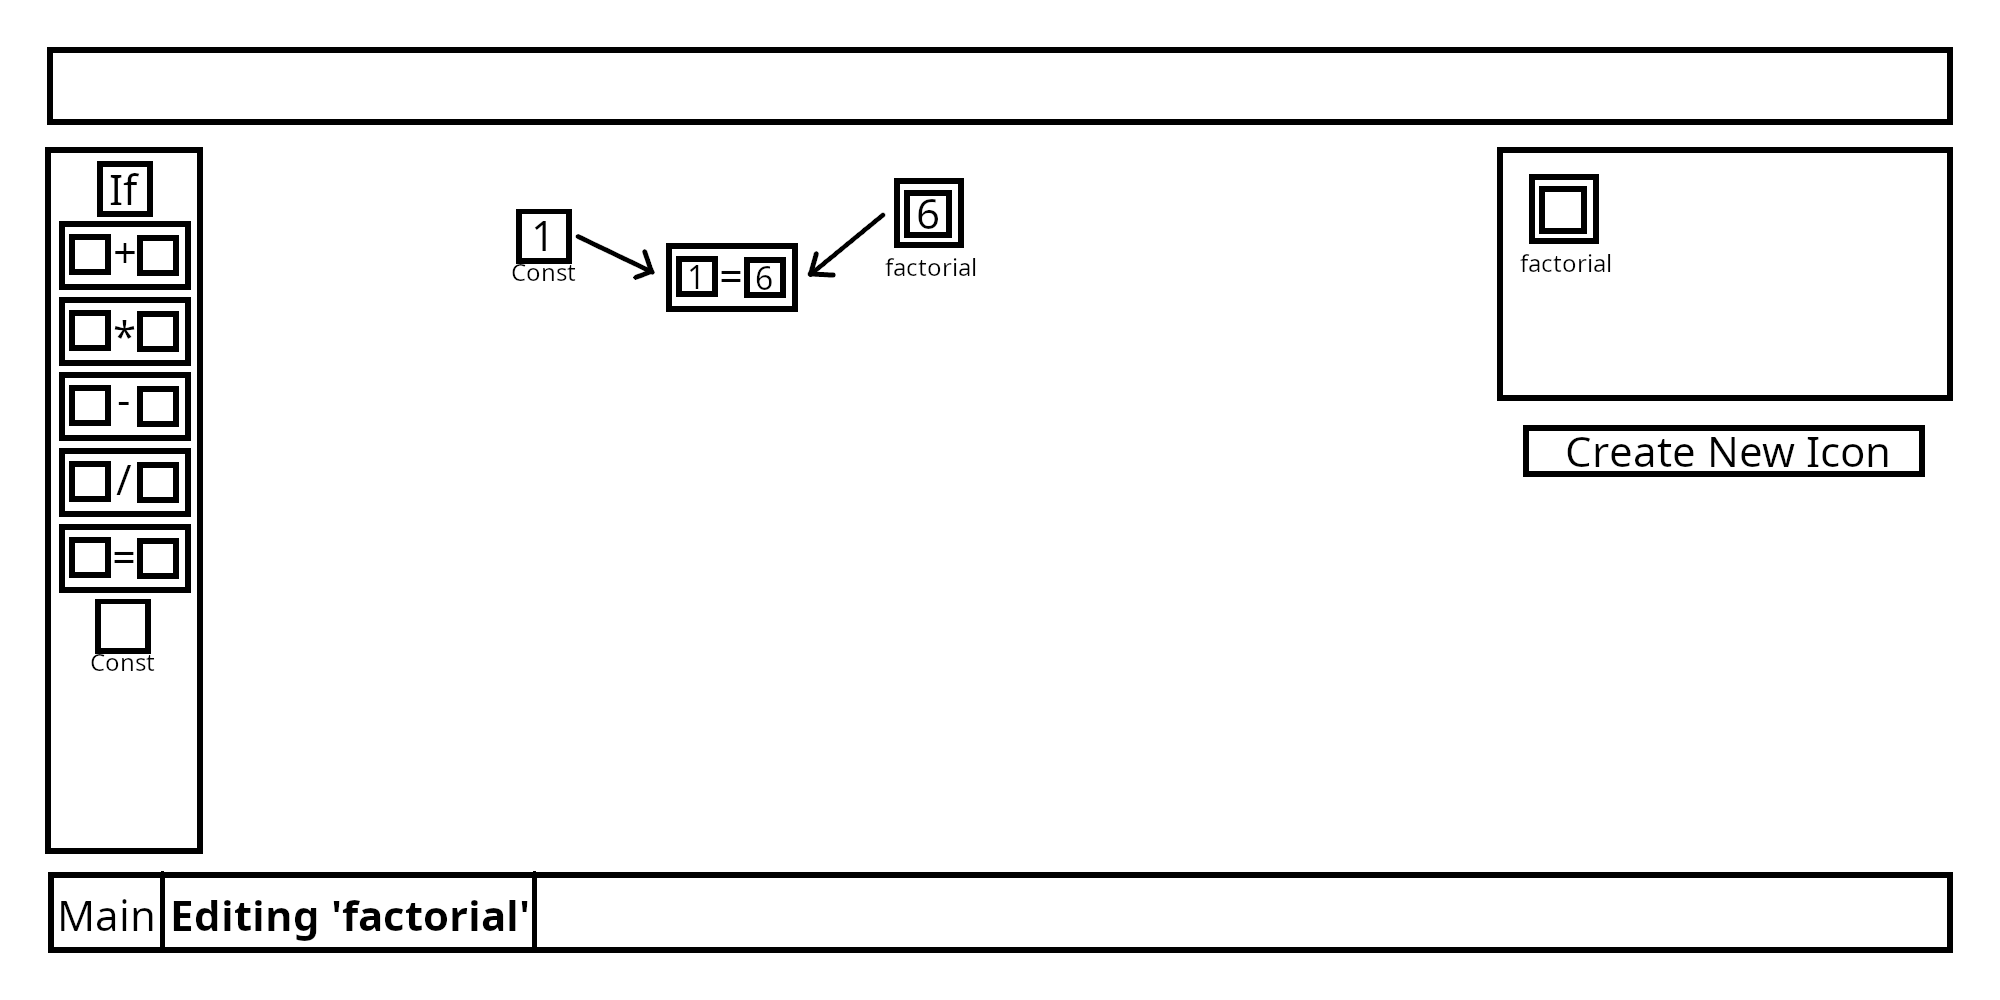
\includegraphics[width=\textwidth]{include/example_factorial_fill_equals.png}
                    \centering
                \end{figure}
                \begin{figure}[H]
                    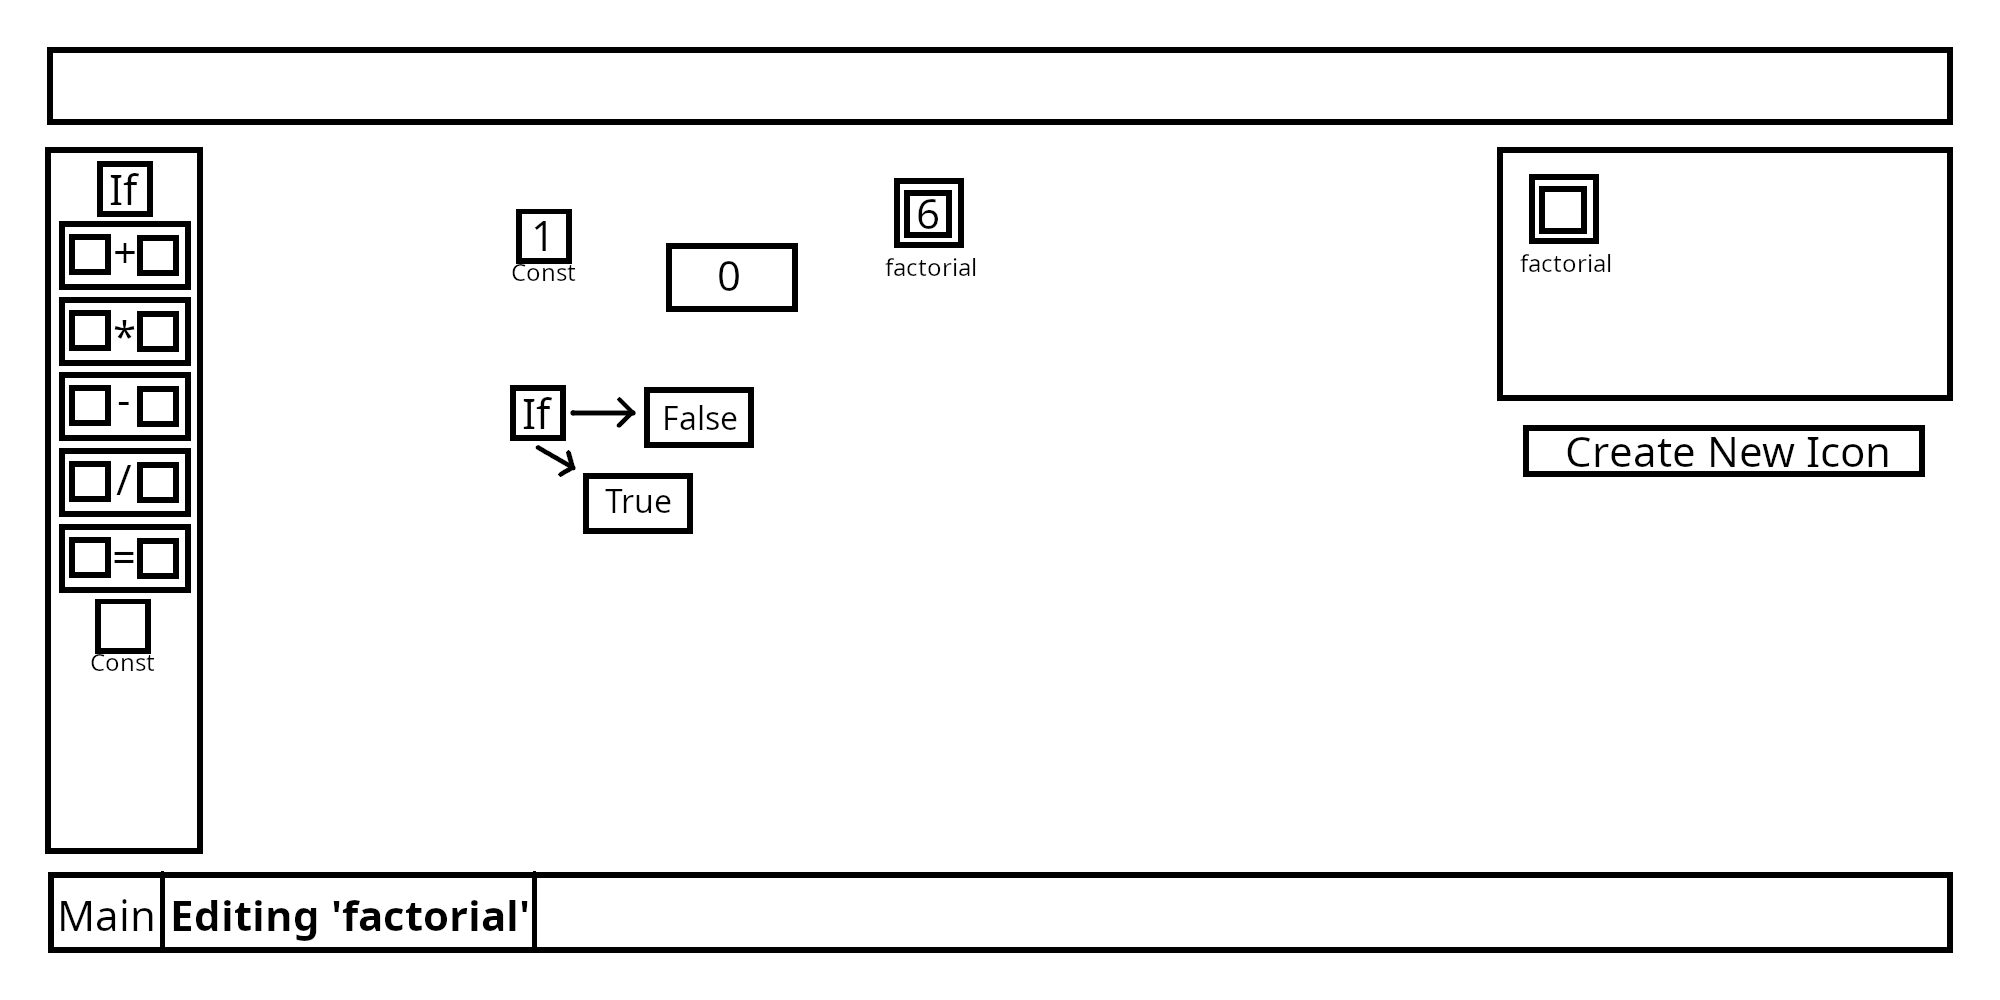
\includegraphics[width=\textwidth]{include/example_factorial_add_if.png}
                    \centering
                \end{figure}
                \begin{figure}[H]
                    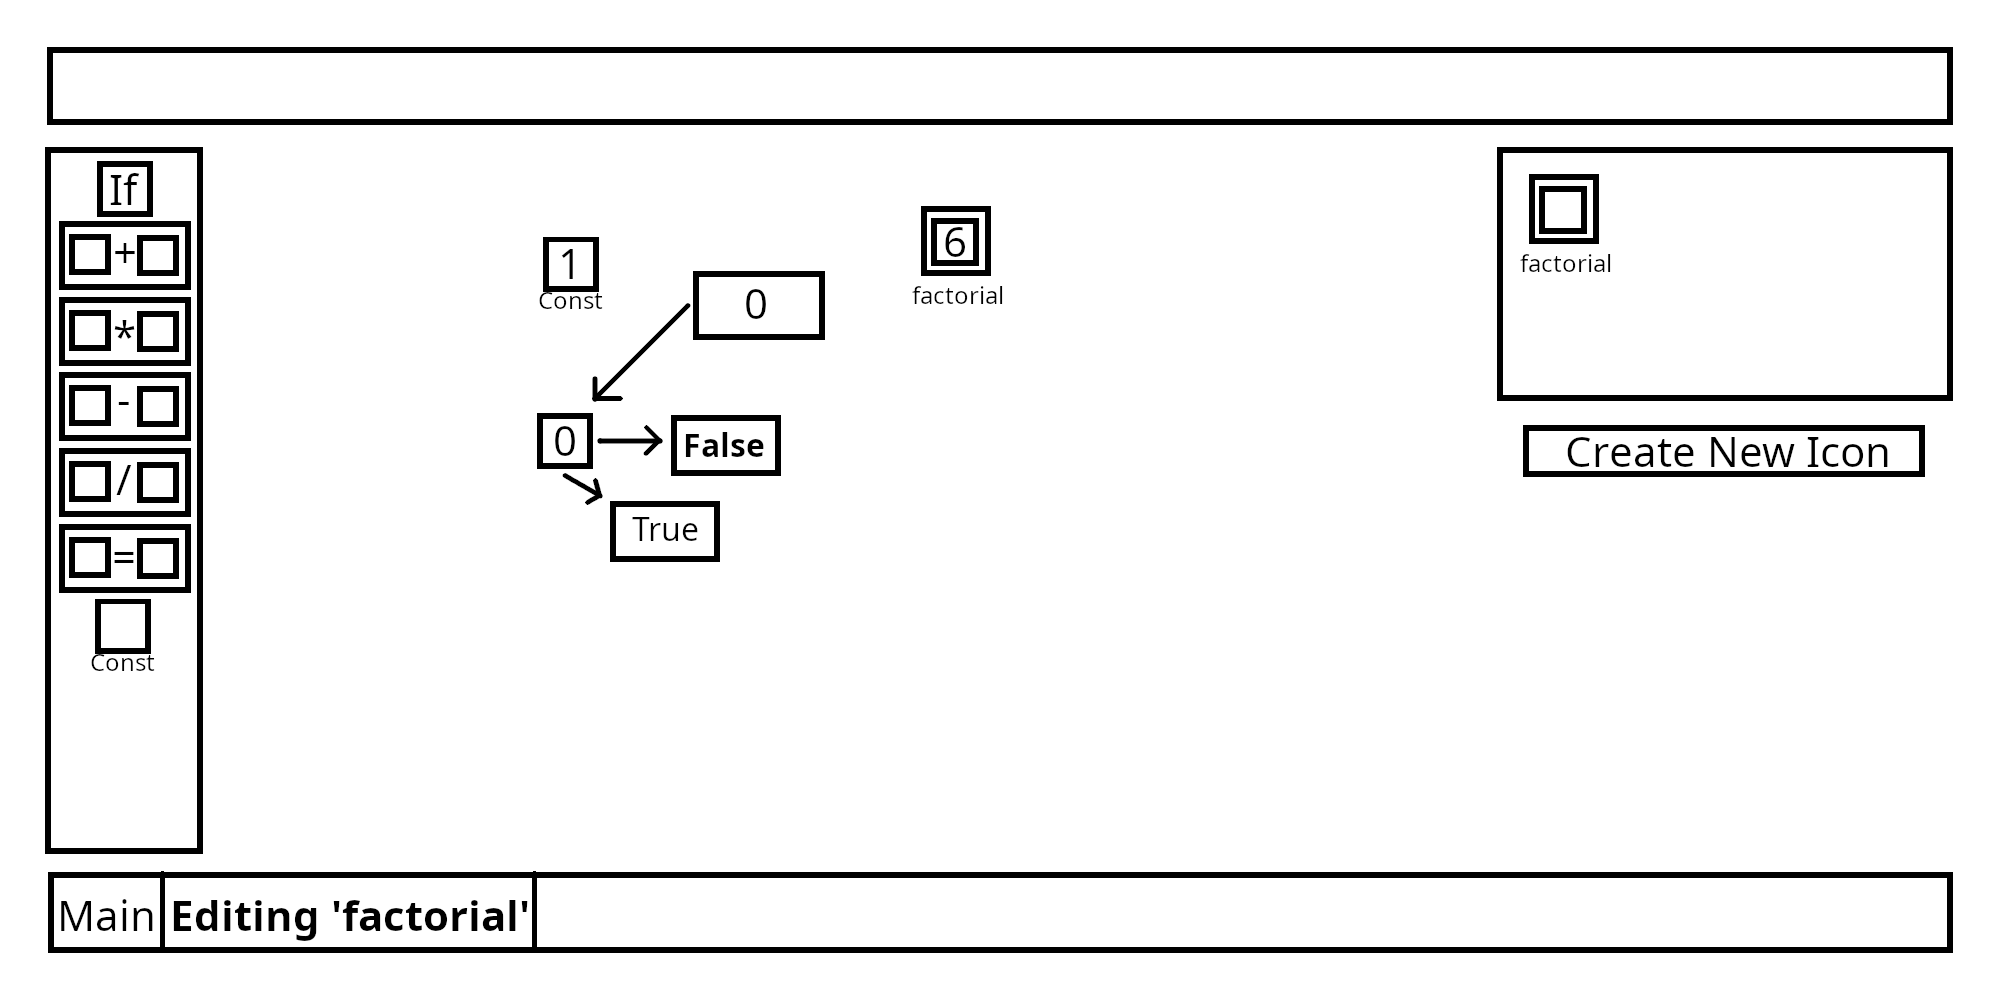
\includegraphics[width=\textwidth]{include/example_factorial_eval_if.png}
                    \centering
                \end{figure}

            \item
                We are writing factorial recursively, so we need to add a new factorial icon to our screen. We then subtract
                one from the input, and drag the result of this operation into the factorial icon. We then left click this icon
                to run it.
                \begin{figure}[H]
                    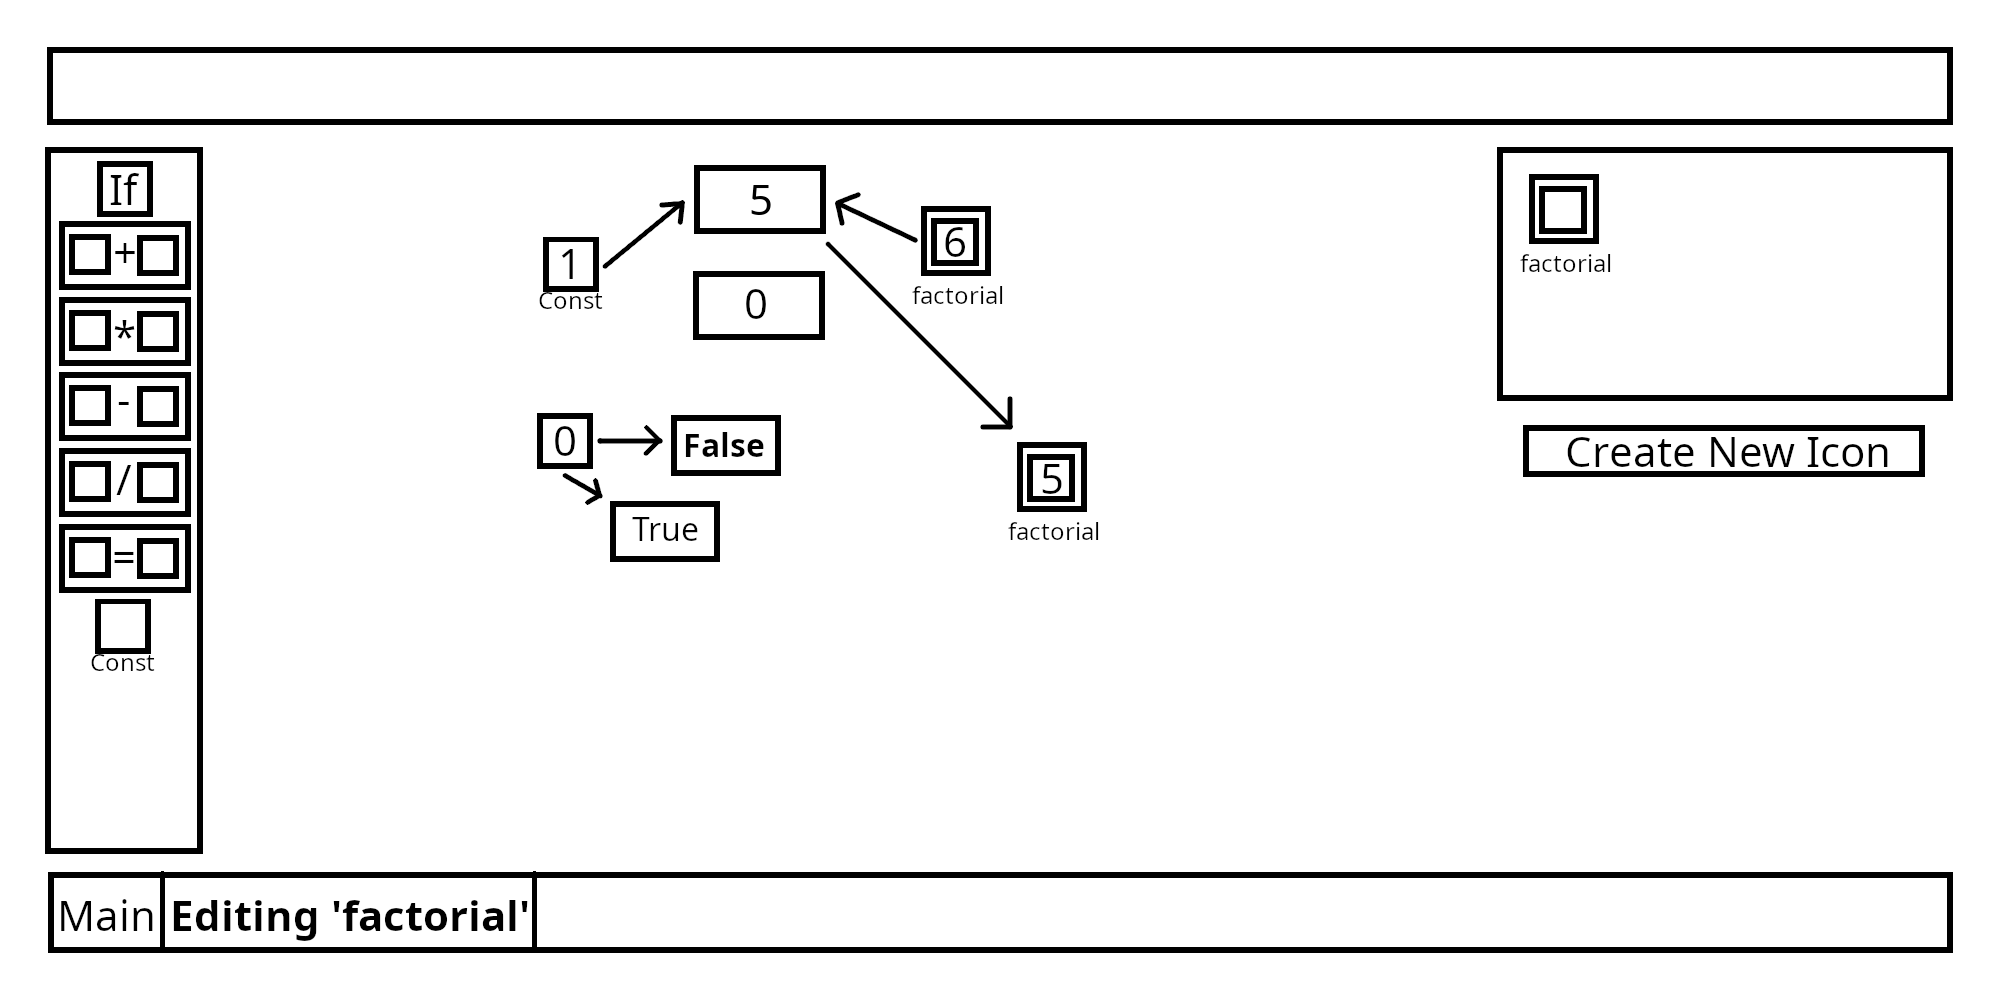
\includegraphics[width=\textwidth]{include/example_factorial_add_next_factorial.png}
                    \centering
                \end{figure}

            \item
                Since we never defined what happens if we execute the \textbf{True} branch, our program hits a \textbf{Trap},
                and it creates a new tab that contains our current status, which means the state where the input is equal to 1.
                We create a new constant block with the value 1, and drag it to the master icon (the first icon that was on
                the screen when we started programming the factorial). This signifies that this value is the output, so running
                the factorial icon with an input of 1 will now actually return a valid value.
                \begin{figure}[H]
                    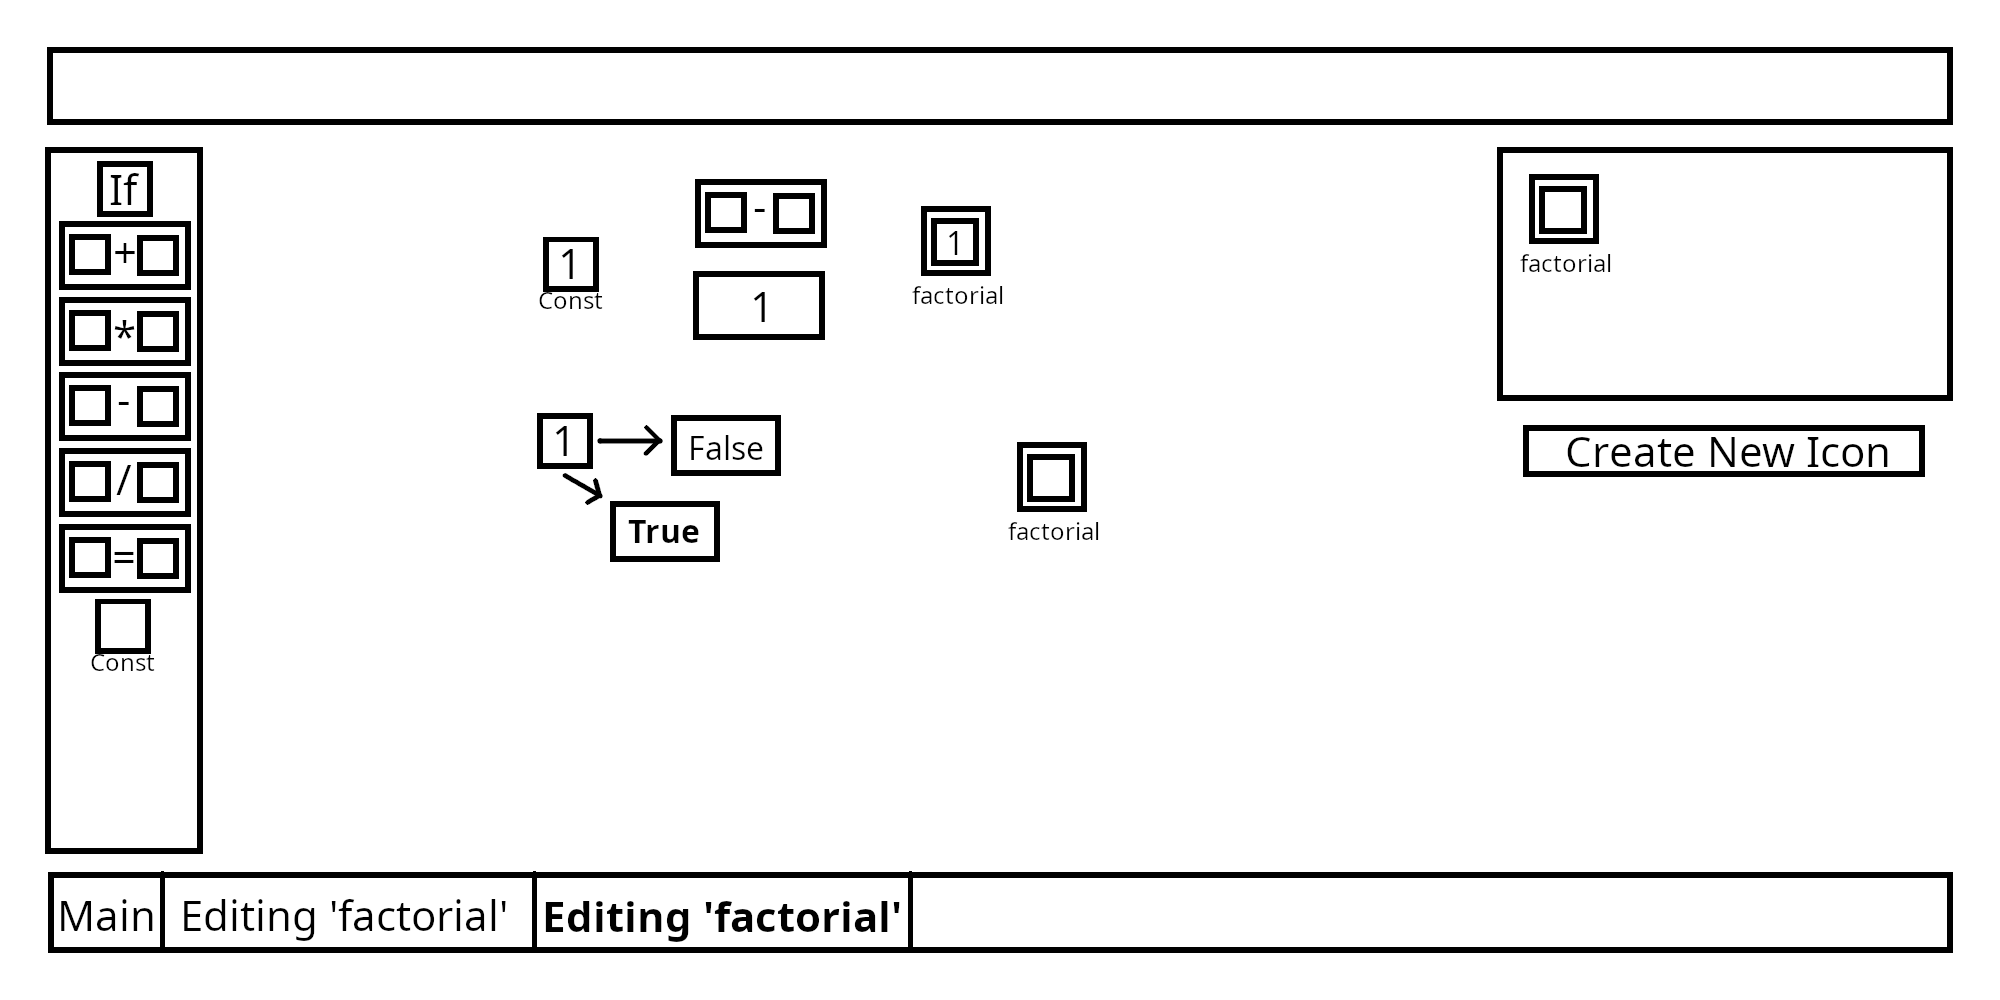
\includegraphics[width=\textwidth]{include/example_factorial_hit_trap_1.png}
                    \centering
                \end{figure}
                \begin{figure}[H]
                    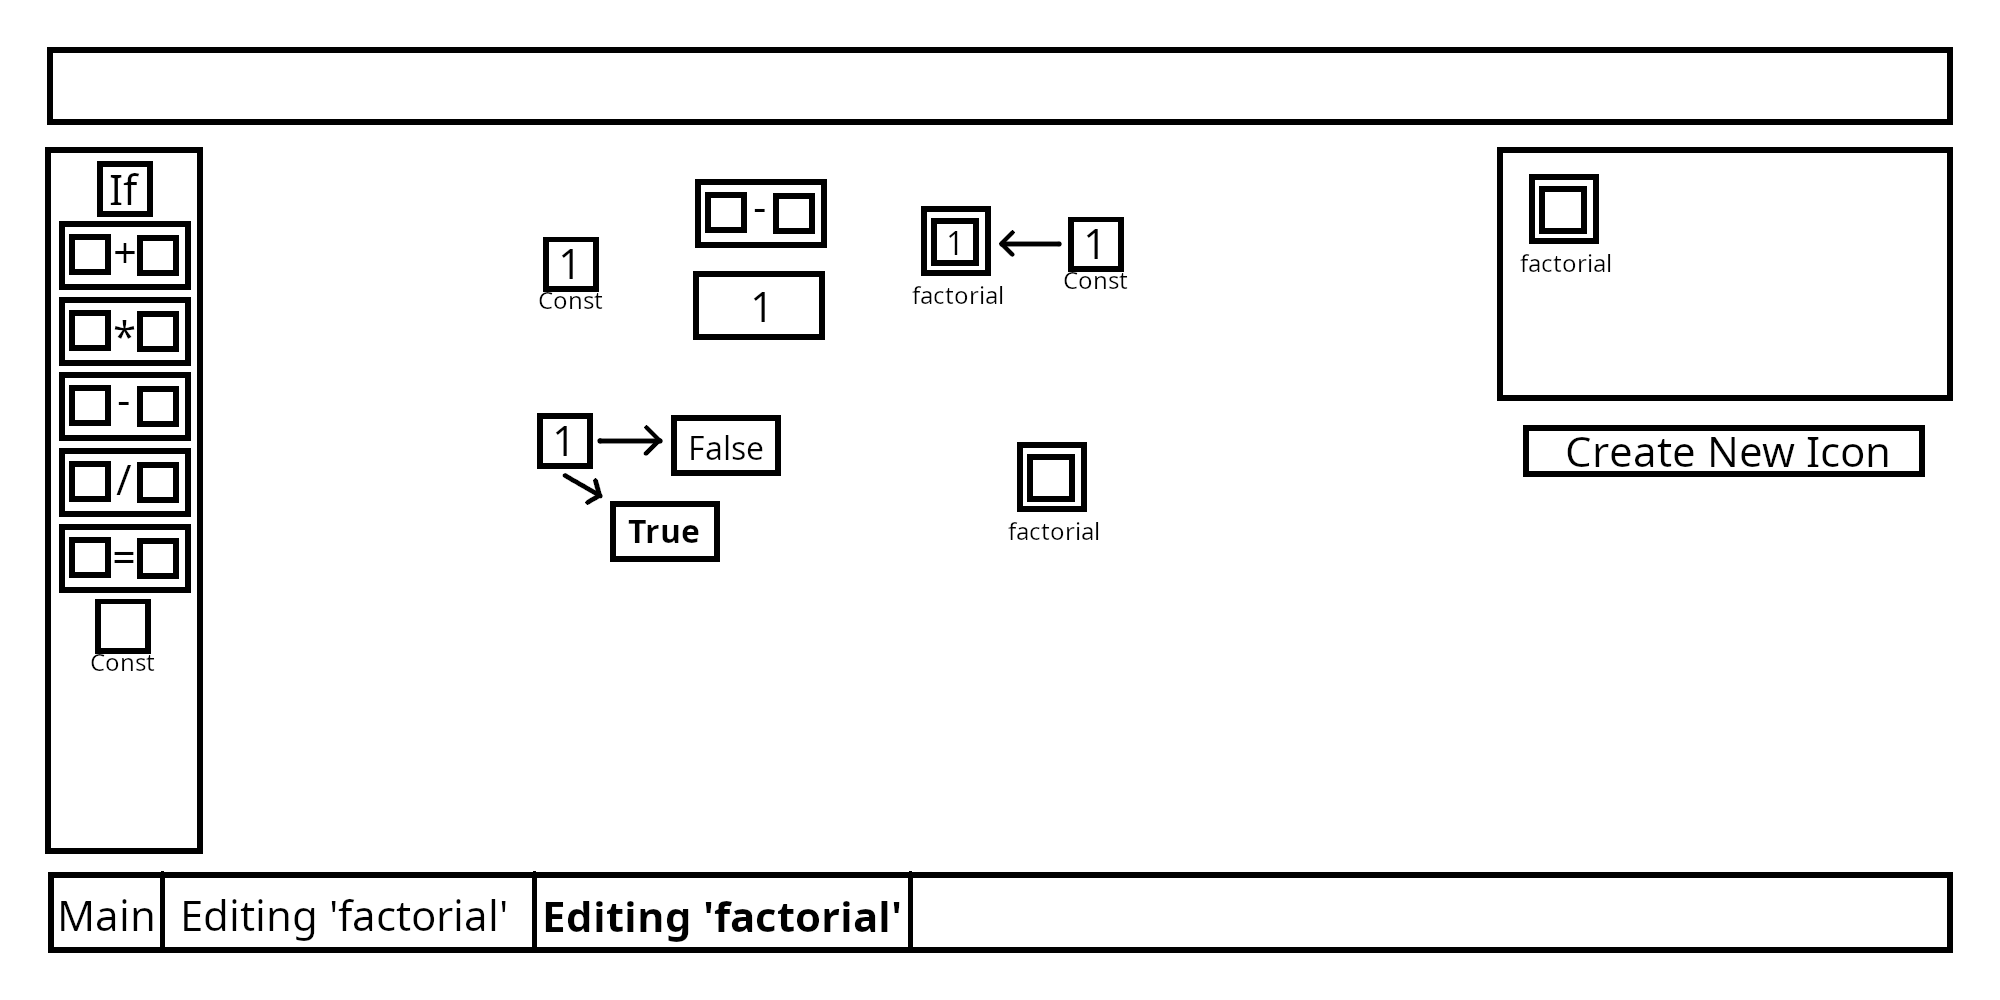
\includegraphics[width=\textwidth]{include/example_factorial_finish_true_branch.png}
                    \centering
                \end{figure}


            \item
                Now we can close this tab and return to our first editing tab. We can see that the changes we made in the other
                tab carried over. We now can try evaluating the factorial again, which will hit another trap, but this time it
                does so because we don't know what to do after evaluating the factorial. We will be put into a new tab where
                the input is 2.
                \begin{figure}[H]
                    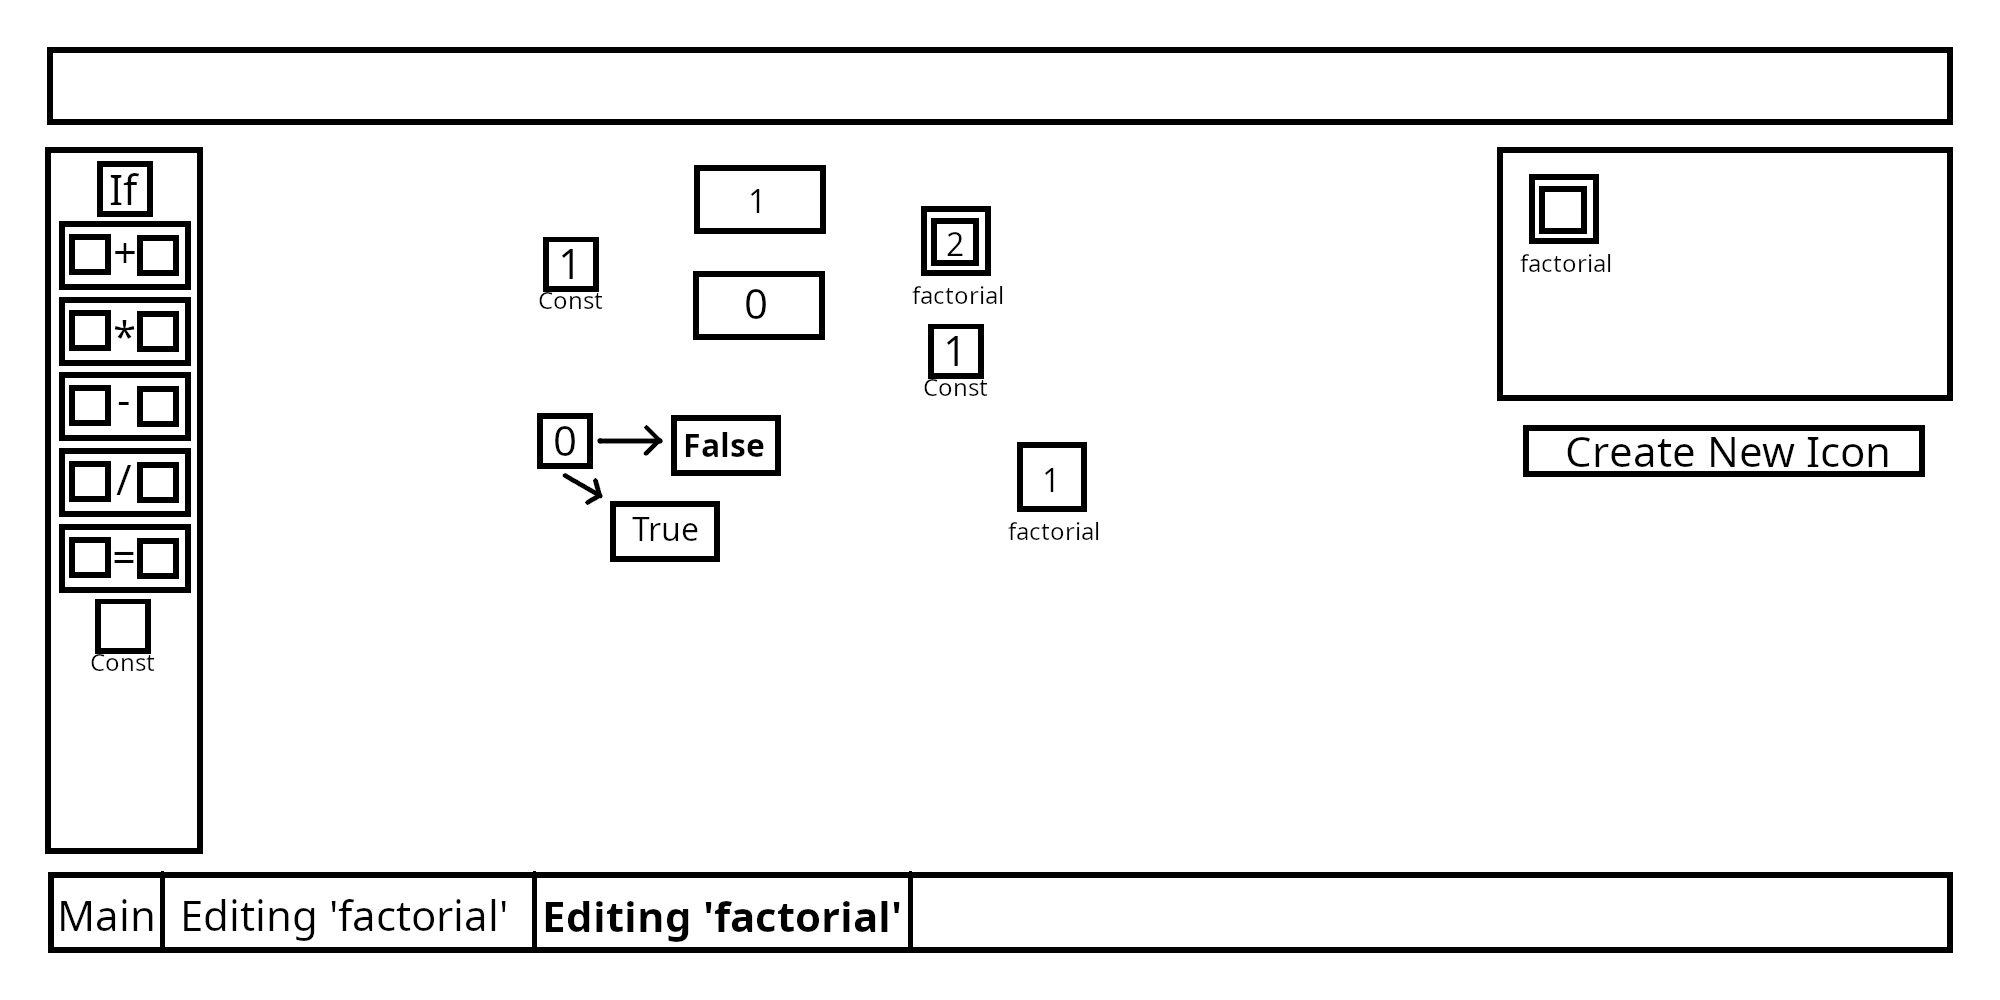
\includegraphics[width=\textwidth]{include/example_factorial_hit_trap_2.png}
                    \centering
                \end{figure}

            \item
                In this tab, we can finally finish the method, by taking the output of the inner factorial, multiplying it with
                our input, and dragging the result into the output. We can now close all new tabs, and our factorial block can
                used.
                \begin{figure}[H]
                    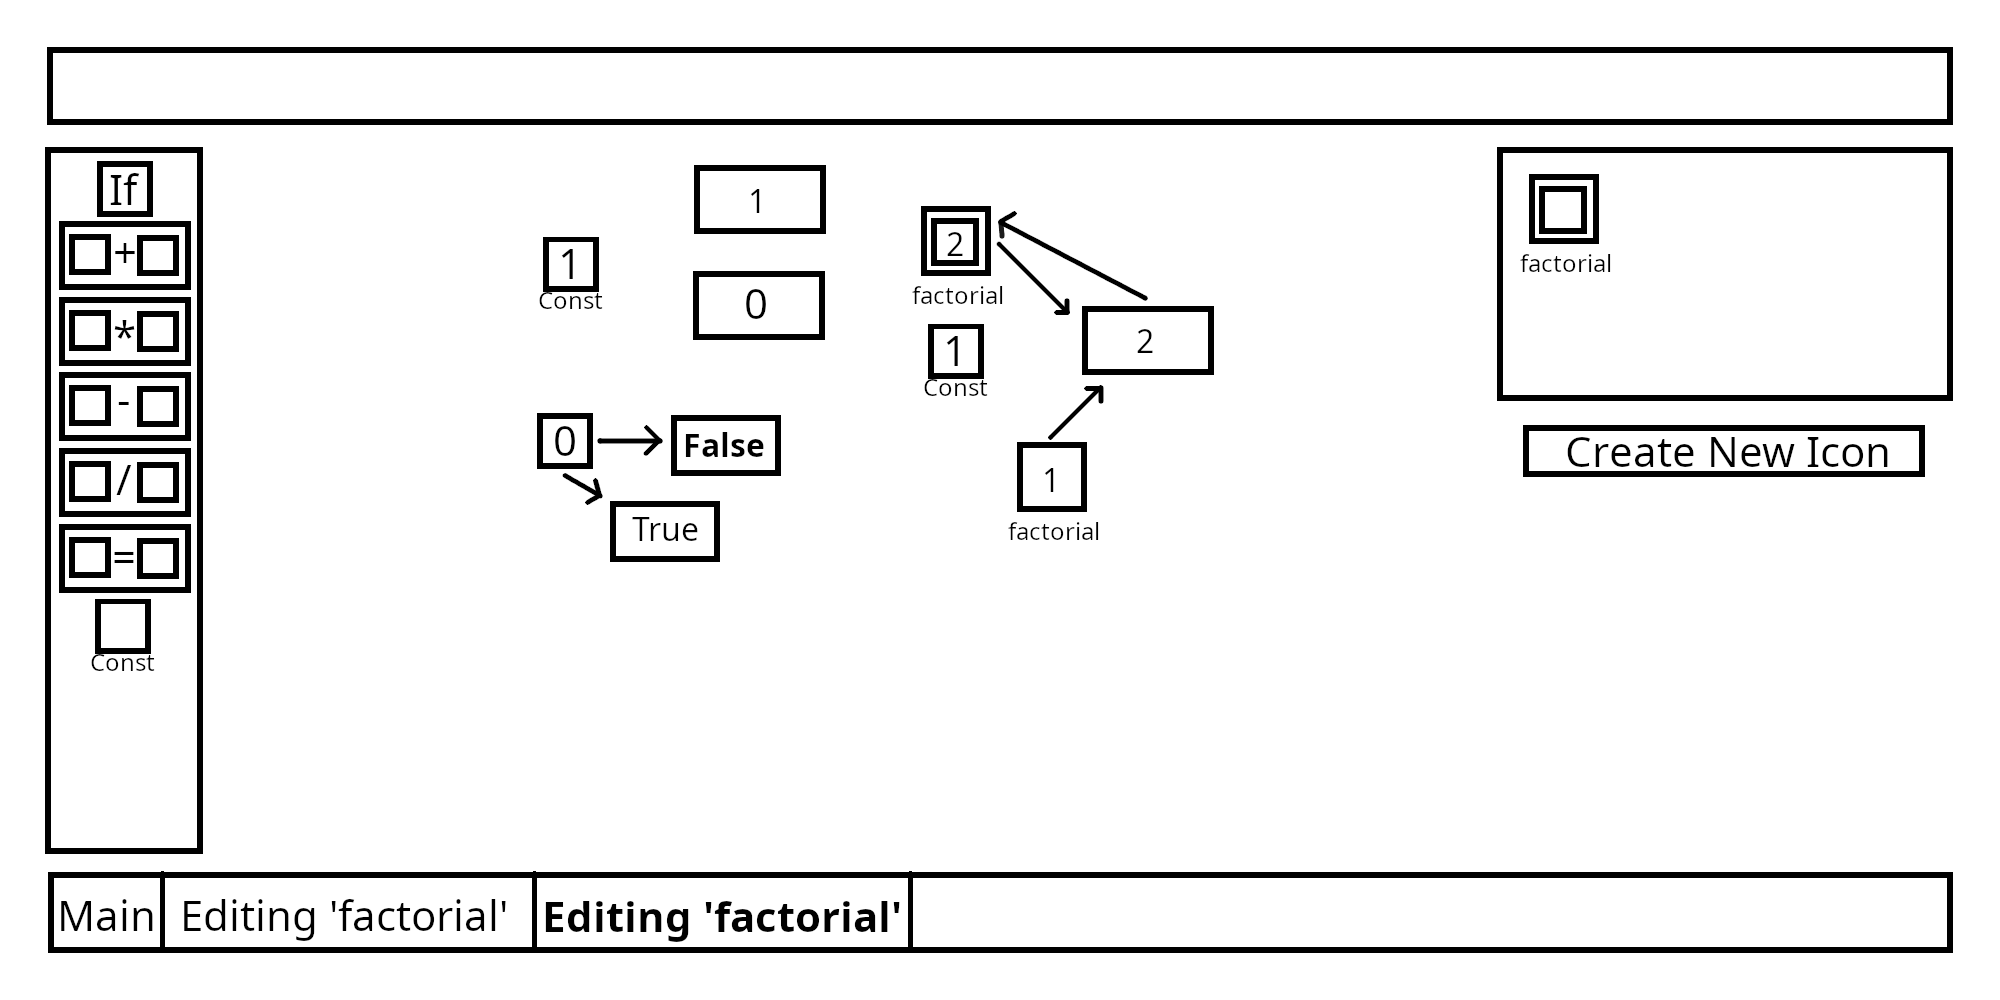
\includegraphics[width=\textwidth]{include/example_factorial_finish_false_branch.png}
                    \centering
                \end{figure}

        \end{itemize}

    \section{Other requirements}
        Because of the fact that this project is a proof of concept, there are not many requirements placed
        on aspects of the project such as performance. The only requirement is that the software works on modern
        browsers, and is responsive.

    \section{Project restrictions}
        \begin{itemize}

            \item
                The only supported type that can be used within the icons are integers. The project may be extended
                to support arbitrary types later on, but for now, this is a non-goal.

            \item
                The icons can only represent pure functions. There is no internal state that can be referenced. This
                means that icons representing data can only exist as functions returning a constant, and that creating
                icons which represent objects is impossible as of now.

        \end{itemize}


    \section{Timeline \& Milestones}
        \begin{tabular}{ | c | c | c | }
            \hline
            Date & Milestone & Presentation method\\
            \hline

            14.05.2023 & First version of documentation & Meeting with supervisor \\

            % Add more milestones after meeting

            \hline

        \end{tabular}


    \addcontentsline{toc}{section}{Appendix A: Terminology}

    \section*{Appendix A: Terminology}


\end{document}
